\documentclass[a4paper, twocolumn]{article}


\usepackage[backend=biber]{biblatex}
%\usepackage[backend=biber, style=authoryear-icomp]{biblatex}
\addbibresource{./refs.bib}

\usepackage{graphicx}

\usepackage{listings}
\usepackage{color}
\definecolor{lightgray}{gray}{0.9}

\lstset{
    showstringspaces=false,
    basicstyle=\ttfamily,
    keywordstyle={blue},
    commentstyle=\color[gray]{0.6},
    stringstyle=\color[RGB]{255, 150, 75}
}
\newcommand{\inlinecode}[2]{\colorbox{lightgray}{\lstinline[language=#1]$#2$}}

%\author{%
%    \begin{tabular}{c@{\hspace{1.5cm}}c}
%        Asmus Skafte Böttcher & Dan Viktor Jørgensen \\
%        {\small\texttt{asbo0001@stud.ek.dk}} & {\small\texttt{danx8076@stud.ek.dk}} \\[10pt]
%        Mathias Frikke Madsen & Wenmin Ye \\
%        {\small\texttt{math64v2@stud.ek.dk}} & {\small\texttt{wenm0007@stud.ek.dk}}
%    \end{tabular}%
%}
\author{%
    \small
    \begin{tabular}{cccc}
        Asmus Skafte Böttcher & Dan Viktor Jørgensen & Mathias Frikke Madsen & Wenmin Ye \\
        \texttt{asbo0001@stud.ek.dk} & \texttt{danx8076@stud.ek.dk} & \texttt{math64v2@stud.ek.dk} & \texttt{wenm0007@stud.ek.dk}
    \end{tabular}%
}

\title{Does Crossover Earn Its Keep? Evolving a Neural Car-Controller with a Genetic Algorithm}



\begin{document}

\twocolumn[
    \begin{@twocolumnfalse}
        \maketitle
        \begin{abstract}
            We develop a small 2D racing game in Python and \texttt{pygame} and train an
            agent to drive it well using a genetic algorithm (GA), without any dataset of
            expert play.
            Each agent is a small feed-forward neural network whose weights
            constitute its genome; the network maps the car's distance sensors to steering
            and throttle.
            Because a GA improves agents through both \emph{crossover} and
            \emph{mutation}, we ask whether crossover actually contributes to learning this
            task, or whether mutation alone performs as well.
            We run an ablation comparing a crossover-plus-mutation GA against an otherwise-identical
            mutation-only GA across multiple independent runs, and test the difference in final fitness for
            statistical significance.
            We find that crossover yields a slightly higher mean final fitness than mutation alone,
            but this gap is driven almost entirely by a small number of runs that fail to converge
            rather than by any difference in the quality of successful controllers, and it is not
            statistically significant at $\alpha = 0.05$. On this task we therefore cannot conclude
            that crossover earns its keep.
        \end{abstract}
    \end{@twocolumnfalse}
    \vspace{1cm}
]


\section{Introduction\label{sec:Introduction}}
Many control problems have no dataset of correct answers to learn from: there is only an
environment in which an agent acts and receives feedback on how well it did, which makes them
a poor fit for ordinary supervised learning \cite{ng2016what}. Driving a car around a track is
one such problem. Rather than hand-coding driving rules, we treat learning to drive as a search
through the space of possible controllers, guided only by a score, and solve it with a
\emph{genetic algorithm} (GA).

Our project consists of two parts. First, we implement a small top-down 2D racing game in
Python using \texttt{pygame}:
a car drives on a closed track and is scored on how far it progresses before crashing or
running out of time.
Second, we replace the human player with a population of artificial agents and evolve them
with a GA, so that good driving behaviour emerges through selection over many generations
rather than being programmed by us.

Each agent is a small feed-forward neural network. Neural networks are a standard and highly
effective model for learning mappings from rich inputs to outputs \cite{lecun2015deep}, and
even a single-hidden-layer network of this kind is expressive enough to approximate the
control function the task requires \cite{leshno1993multilayer}. Its inputs are
the car's sensor readings, and its outputs are the driving controls. Following the standard
GA terminology, the network's weights form the \emph{genome} (the genotype), while the driving
behaviour those weights produce is the \emph{phenotype}. The GA never sees the track directly;
it only sees how fit each genome's behaviour turns out to be.

A GA improves a population using three operators: selection, \emph{crossover} (recombination
of two parents, analogous to sexual reproduction), and \emph{mutation} (small random changes).
Crossover is often assumed to be a central driver of a GA's performance, yet for some problems
mutation-only (``asexual'') evolution does just as well. Whether crossover helps is therefore
an empirical question, and it is the question this paper investigates for our racing task.

We also note that GAs are closely related to reinforcement learning: both learn from
environment feedback rather than from a labelled dataset. A GA maintains a whole population of
candidate solutions, which makes it less likely to get stuck in a local optimum than a single
model trained in isolation. We use a GA in this work and leave a direct comparison with
reinforcement learning for future work.


\subsection{Problem Formulation\label{sec:Problem Formulation}}

We formulate the problem as a pair of hypotheses to be tested. The \emph{independent
variable} ($X$) that we manipulate is the reproduction strategy, with two levels:
(i) crossover combined with mutation, and (ii) mutation only. The \emph{dependent variable}
($Y$) that we measure is the final fitness, defined as the best fitness in the population at
the final generation, recorded across a number of independent runs. All other parameters are
held constant between the two levels.

\begin{quote}
\textbf{H\textsubscript{1} (alternative):} A genetic algorithm using both crossover and
mutation evolves car-controllers with a higher mean final fitness than an
otherwise-identical genetic algorithm using mutation only.
\end{quote}

\begin{quote}
\textbf{H\textsubscript{0} (null):} There is no systematic difference in mean final fitness
between the two reproduction strategies; any observed difference is due to chance alone.
\end{quote}

Following standard practice in inferential statistics, we do not attempt to ``prove''
H\textsubscript{1}; instead we test whether the evidence is strong enough to \emph{reject}
H\textsubscript{0}.

\section{Methods\label{sec:Methods}}

Our work follows an agile, multi-methodological research process in the sense of
\textcite{nunamaker1990systems}, moving repeatedly between theory building (GA theory),
systems development (the game and the GA), observation (logging fitness during training), and
experimentation (the ablation described below). To keep the work transparent and reproducible,
every step from environment configuration to the final statistical test is scripted and driven
by fixed random seeds and a single configuration file; no results are produced by manual
interaction.


\subsection{Environment and Agent Interaction\label{sec:Environment}}

The environment is the racing game. On each simulation step the agent receives a fixed-length
vector of inputs and returns a fixed-length vector of actions.


\begin{itemize}
    \item \textbf{Inputs (sensors).} The car casts three rays at fixed angles relative to its heading.
    at fixed angles relative to its heading (Figure~\ref{fig:car_with_sensors}); each ray returns the normalised distance to the
    nearest track edge. We optionally include the car's current speed as an additional input.
    \item \textbf{Outputs (actions).} The network produces two values: a steering signal in
    $[-1, 1]$ and a throttle signal.
\end{itemize}

\begin{figure}[ht]
    \centering
    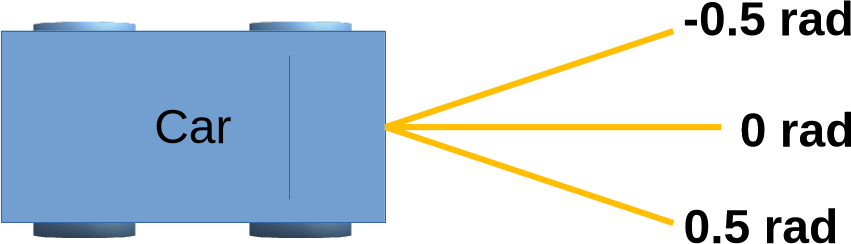
\includegraphics[width=0.9\columnwidth]{figures/car_with_senors.png}
    \caption{The car's distance sensors. Three rays are cast at fixed angles
    ($-0.5$, $0$, $+0.5$ radians, i.e. $\approx -28.6^\circ$, $0^\circ$, $+28.6^\circ$) relative to the car's
    heading; each ray returns the normalised distance to the nearest track edge.}
    \label{fig:car_with_sensors}
\end{figure}

The mapping from inputs to outputs is a small feed-forward neural network with four inputs,
one hidden layer of six units, and two outputs, using $\tanh$ activations throughout
($4 \to 6 \to 2$). % NOTE: from network.py.
The genome is the flat vector of all $4\times 6 + 6\times 2 = 36$ connection weights; the network
uses no bias terms, so an agent is fully specified by these 36 weights.
This is the genotype/phenotype distinction in concrete form:
the weight vector is the genotype, and the resulting trajectory of the car is the phenotype.

\subsection{Fitness Function\label{sec:Fitness}}
Fitness accumulates over the simulation steps of a run. At each step the agent receives a small
reward proportional to its current speed and a small constant penalty for not advancing
(discouraging standing still). The track is divided by an ordered sequence of checkpoints
(gates); crossing the next expected gate awards a bonus that grows with the gate index, so
progressing further is worth more. Completing the required number of laps awards a large
one-off completion bonus and ends the run. A run also ends when the car crashes, when it fails
to reach a new checkpoint within a timeout, or when a hard step limit is reached.
We deliberately reward ordered checkpoint progress rather than raw distance travelled, because
the latter encourages degenerate behaviour such as driving in tight circles.
% NOTE: See world.py and train_ai.py

\subsection{Genetic Algorithm Design\label{sec:GA Design}}

We initialise a population of $N = 35$
agents with random weights, then repeat the following each generation until a fixed generation
budget is reached:

\begin{enumerate}
    \item \textbf{Evaluation.} Each agent drives the track and receives a fitness score
    (Section~\ref{sec:Fitness}).
    \item \textbf{Selection.} We sort the population by fitness and retain the fitter
    individuals as parents. We apply \emph{elitism}: the three best agents are copied unchanged
    % NOTE: elitism_count can be changed in comfig
    into the next generation so strong solutions are never lost to chance.
    \item \textbf{Reproduction.} New offspring are produced from selected parents using the
    reproduction strategy under test (Section~\ref{sec:Experimental Design}), then mutated.
\end{enumerate}

The genetic operators are adapted to a real-valued genome. Parents are chosen by
\emph{tournament selection} (the fittest of five randomly sampled agents). \emph{Crossover} is
uniform: each child weight is taken independently from one parent or the other with equal
probability. \emph{Mutation} then visits each weight and, with probability equal to the mutation
rate $0.1$, adds Gaussian noise of standard deviation $0.5$.
% NOTE: See genetic_algorithm.py

\subsection{Experimental Design\label{sec:Experimental Design}}

To test the hypotheses we run an \emph{ablation}: the only thing that changes between
conditions is the reproduction strategy (the independent variable $X$).

\begin{itemize}
    \item \textbf{Condition A (crossover + mutation).} Offspring are produced by crossover of
    two parents and then mutated.
    \item \textbf{Condition B (mutation only).} Offspring are exact copies of a single selected
    parent and then mutated; no crossover occurs.
\end{itemize}

Population size ($N=35$), number of generations ($20$), network architecture, selection scheme,
mutation rate, track, and evaluation budget are held identical across the two conditions. Because
a GA is stochastic, a single run proves nothing, so we run $30$
independent runs per condition with different random seeds, and log the best and mean fitness
at every generation.


\subsection{Analysis Plan\label{sec:Analysis Plan}}

For each condition we obtain a distribution of final-fitness values $Y$ (one value per run).
We compare the two conditions both visually and statistically. Visually, we plot mean
best-fitness per generation for both conditions with a band showing the spread across runs.
Statistically, we test the difference in final fitness between the two independent groups.
Since the fitness values may not be normally distributed, we use a non-parametric two-sample
test (the Mann--Whitney U test \cite{mann1947test}); if the normality assumption is reasonable
an independent two-sample $t$-test is an alternative. We set the significance level to
$\alpha = 0.05$ and reject H\textsubscript{0} if the resulting $p$-value is below $\alpha$,
keeping in mind the risk of Type~1 and Type~2 errors. The analysis itself is presented in
Section~\ref{sec:Analysis}.

\section{Analysis\label{sec:Analysis}}
% TODO: apply the methods. Show the training curves and run the statistical test.
% Cross-reference back to Section~\ref{sec:Methods}.

We apply the plan of Section~\ref{sec:Analysis Plan} to the $30$ runs per condition.
Figure~\ref{fig:learning_curve} shows the mean best-fitness per generation for both
conditions, with a band of $\pm 1$ standard deviation across runs. The two trajectories rise
together and remain heavily overlapped throughout: at no generation does either condition
separate from the other beyond its run-to-run spread, and both are still climbing at the final
generation rather than having plateaued.

\begin{figure}[ht]
    \centering
    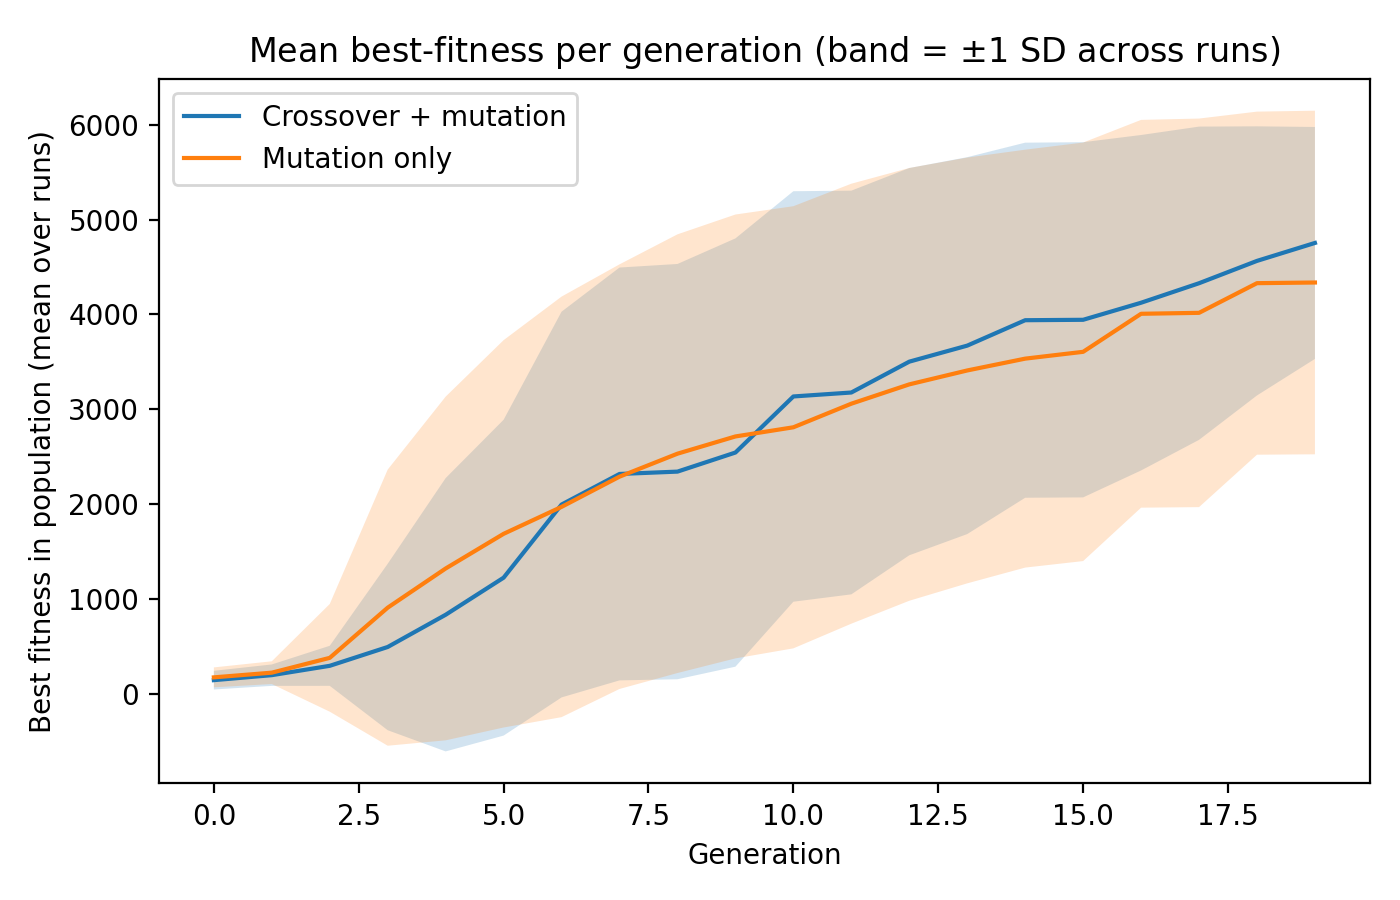
\includegraphics[width=\columnwidth]{figures/learning_curve.png}
    \caption{Mean best-fitness in the population per generation, averaged over the $30$ runs of
    each condition; the shaded band is $\pm 1$ standard deviation across runs. The conditions
    overlap throughout and are still rising at generation~$20$.}
    \label{fig:learning_curve}
\end{figure}

We then test the final-fitness values statistically using the pre-registered Mann-Whitney U
test \cite{mann1947test}. Inspecting the final-fitness values revealed that their distribution
is strongly bimodal: most runs converge to a tight cluster around fitness~$5100$, while a small
number fail to converge within $20$ generations and score far lower, with a clear gap between
the two groups. Because a mean over a bimodal distribution conflates ``how often a method
solves the task'' with ``how good its solutions are,'' we additionally report two exploratory,
post-hoc analyses: a comparison of \emph{convergence rate} (Fisher's exact test on the number of
converged runs) and a comparison of \emph{solution quality among converged runs only} (a second
Mann--Whitney U test). A run is counted as converged if its final fitness lies in the upper
cluster; the gap between clusters is wide enough that the exact cut-off does not affect the
counts.

\section{Findings\label{sec:Findings}}
% TODO: present results only, no interpretation. Report the test statistic and p-value,
% and cross-reference back to Section~\ref{sec:Analysis}.

\paragraph{Final fitness (pre-registered test).}
The crossover condition reached a mean final fitness of $4753.5$ (SD $1221.7$) and the
mutation-only condition $4336.6$ (SD $1810.2$). The two-sided Mann--Whitney U test gives
$U = 472.0$, $p = 0.75$, with a rank-biserial effect size of $-0.05$. A Welch two-sample
$t$-test agrees ($t = 1.05$, $p = 0.30$). At $\alpha = 0.05$ we fail to reject
H\textsubscript{0}.

\paragraph{Convergence rate (exploratory).}
The crossover condition converged in $27$ of $30$ runs and the mutation-only condition in $25$
of $30$ (Table~\ref{tab:convergence}). A two-sided Fisher's exact test gives an odds ratio of
$1.80$ and $p = 0.71$.

\begin{table}[ht]
    \centering
    \small
    \begin{tabular}{lcc}
        \hline
        Condition & Converged & Rate \\
        \hline
        Crossover + mutation & $27/30$ & $90\%$ \\
        Mutation only        & $25/30$ & $83\%$ \\
        \hline
    \end{tabular}
    \caption{Number of runs reaching the converged cluster, per condition.
    Fisher's exact test: $p = 0.71$.}
    \label{tab:convergence}
\end{table}

\paragraph{Solution quality among converged runs (exploratory).}
Restricted to converged runs, the two conditions are near-identical
(Table~\ref{tab:quality}): mean final fitness $5120.6$ (SD $104.3$, $n = 27$) for crossover and
$5130.1$ (SD $110.2$, $n = 25$) for mutation only. A two-sided Mann--Whitney U test on these
values gives $p = 0.84$.

\begin{table}[ht]
    \centering
    \small
    \begin{tabular}{lcccc}
        \hline
        Condition & $n$ & Mean & SD & Range \\
        \hline
        Crossover + mut. & $27$ & $5120.6$ & $104.3$ & $4945$--$5308$ \\
        Mutation only    & $25$ & $5130.1$ & $110.2$ & $4944$--$5370$ \\
        \hline
    \end{tabular}
    \caption{Final fitness of converged runs only. Mann--Whitney U: $p = 0.84$.}
    \label{tab:quality}
\end{table}


\section{Conclusion\label{sec:Conclusion}}
% TODO: answer the research question / hypotheses based on the findings. Here you may
% interpret. Cross-reference Sections~\ref{sec:Problem Formulation}, \ref{sec:Analysis},
% and \ref{sec:Findings}.

Our experiment fails to reject the null hypothesis H\textsubscript{0}
(Section~\ref{sec:Problem Formulation}): 
on this racing task, a genetic algorithm using
crossover and mutation did not achieve a significantly higher final fitness than an
otherwise-identical mutation-only algorithm ($p = 0.75$, Section~\ref{sec:Findings}).

The decomposition in Section~\ref{sec:Findings} explains where the apparent mean advantage of
crossover comes from.
The two methods are statistically indistinguishable among runs that solve the track ($p = 0.84$),
and crossover's small edge in convergence rate is not significant either ($p = 0.71$).
The $\sim\!420$-point gap in raw means is therefore an artefact of a few extra
non-converging runs in the mutation-only condition, not evidence that crossover produces better
controllers.

This result should be read together with two limitations of the experiment as run.
First, the fitness function awards a large flat bonus on lap completion
(Section~\ref{sec:Fitness}), so every successful controller saturates at essentially the same
score; the experiment therefore has little power to detect a quality difference between methods
even if one exists, because the metric has no headroom above ``solved the track.''
Second, both conditions are still improving at the final generation (Figure~\ref{fig:learning_curve}),
so the comparison is taken before either method has converged, where a late-emerging effect
of crossover would be missed.

A stronger follow-up experiment would (i) replace the flat completion bonus with a reward that
keeps separating controllers after they finish, for example by lap time, so that solution
quality has room to vary; (ii) extend the generation budget until the learning curves plateau;
and (iii) adopt a paired design in which both conditions share each run's initialisation seed
and differ only in whether crossover is applied, analysed with a Wilcoxon signed-rank test,
which removes between-run variance and tests the same hypothesis with more power.
Within the present task and budget, however, the evidence does not support the claim that
crossover earns its keep.

\printbibliography

\end{document}
